 \begin{figure}[h] 
        \centering 
        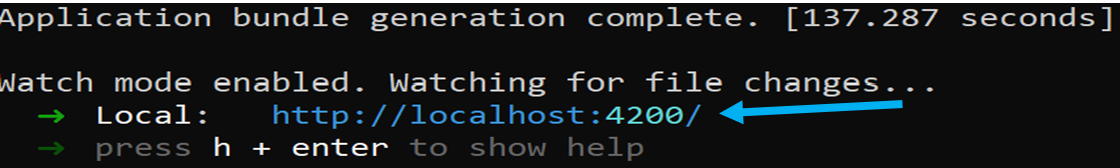
\includegraphics[width=0.8\textwidth]{./img/angular.png} 
    \end{figure}



\documentclass[12pt]{article}
\usepackage[utf8]{inputenc}
\usepackage[T1]{fontenc}
\usepackage[french]{babel}
\usepackage{geometry}
\usepackage{listings}
\usepackage{xcolor}
\usepackage{graphicx}
\usepackage{hyperref}
\usepackage{enumitem}
\usepackage{titlesec}

\geometry{a4paper, margin=2.5cm}

\lstset{
    basicstyle=\ttfamily,
    backgroundcolor=\color{gray!10},
    frame=single,
    breaklines=true
}

\title{Guide complet pour la prise en main de notre application d’aide à l’archivage et à la consultation des projets de fin d'année des étudiants.}
\author{Ange FOKAM, PELAP Amelie-Laure}
\date{30/06/2025}

\begin{document}

\maketitle
\clearpage

\tableofcontents
\clearpage

% -------------------------------
\textbf{\textit{Pour les développeurs et les administrateurs système}}

\rule{\linewidth}{0.2pt}
\section*{À propos du guide :}
\addcontentsline{toc}{section}{À propos du guide}

\begin{itemize}[label=--]
    \item \textbf{Objectif du guide} : Expliquer comment acquérir les logiciels nécessaires et procéder au déploiement proprement dit de l'application.
    \item \textbf{Public cible} : Administrateurs système futurs et développeurs futurs de l'application.
    \item \textbf{Structure du document} : Deux sections à savoir une pour le matériel à disposer et l'autre pour le déploiement technique de l'application.
    \item \textbf{Prérequis généraux} : Accès au réseau internet, identifiants, connaissances de base en informatique et en programmation web ou mobile.
\end{itemize}

\rule{\linewidth}{0.2pt}

\vfill
\rule{\linewidth}{0.2pt}
\textbf{\textit{Ce guide a pour objectif de rendre l’utilisation et la maintenance de l’application aussi claires et simples
que possible. En suivant les étapes décrites, les développeurs pourront exploiter pleinement l'application tout en s'assurant de sa 
pérennité et de son efficacité.}}

\newpage

% Introduction
{\fontsize{14}{16}\section*{Introduction}}
\addcontentsline{toc}{section}{Introduction}
Dans le monde du développement, les applications doivent être en constante évolution pour rester en vogue sur le marché. Par conséquent, elles doivent être conçues de manière à ce que les générations futures puissent
facilement assurer leur maintenance et leur mise à jour. À cet effet, nous avons mis sur pied une série d'étapes pour le lancement de notre application
à partir d’un poste personnel, afin de faciliter la compréhension et la maintenance par les
développeurs et administrateurs. Bien que ce processus puisse sembler complexe, il vise à faciliter la prise en main et la
maintenance à long terme de l’application par les futurs intervenants; ainsi que la gestion
des projets de fin d'études des étudiants. Pour un déploiement complet de l'application, nous avons réparti la présentation en cinq
parties. La première portera sur la présentation du matériel nécessaire, la deuxième sur le procédé d'installation des différents environnements, la troisième montrera comment modifier les variables d'environnement. Les quatrième et cinquième parties porteront sur le déploiement des serveurs et l'ouverture de l'application respectivement.

\vspace{0.5cm}
\rule{\linewidth}{0.2pt}

\newpage
% Guide de déploiement
{\fontsize{14}{16}\section*{Guide de déploiement de l’application}}
\addcontentsline{toc}{section}{Guide de déploiement de l’application}
\setcounter{subsection}{0} % On remet la numérotation des sections à zéro
\renewcommand\thesubsection{\arabic{subsection}}
\rule{\linewidth}{0.2pt}
\subsection{Prérequis}
\textbf{Logiciels nécessaires :}

Avant tout, assurez-vous d'avoir installé les logiciels suivants:

\begin{itemize}[label=--]
    \item PHP (version 8.0 ou plus récente)
    \item Composer(un gestionnaire de dépendances pour PHP)
    \item Angular (framework JavaScript)
    \item Laravel 10 (ou une version plus récente, comme framework PHP)
    \item VS Code(comme éditeur de texte)
    \item MySQL (via XAMPP ou autre,comme SGBD)
    \item Elasticsearch (version compatible )
    
\end{itemize}
\rule{\linewidth}{0.2pt}
\textbf{Configuration minimale recommandée :}

Pour votre poste de travail, il faut:

\begin{itemize}[label=--]
    \item Processeur : 2 GHz double cœur ou plus
    \item RAM : 8 Go minimum
    \item Espace libre sur le disque dur: 30 Go minimum
\end{itemize}
\rule{\linewidth}{0.2pt}
\textbf{Outils supplémentaires :}

\begin{itemize}[label=--]
    \item outil de versioning(GIT de préférence, avec un compte GitHub pour la collaboration)
    \item Accès à Internet (via un FAI ou un VPN)
    \item Navigateur web à jour (Chrome, Firefox, Microsoft Edge, Opera, etc.)
\end{itemize}
\rule{\linewidth}{0.2pt}
\subsection{Étapes de déploiement}

Voici les étapes pour l’ouverture du projet (for windows and Linux):

\begin{enumerate}
    \item \textbf{Cloner le dépôt GitHub}

Lien du dépôt :
        \begin{lstlisting}
git clone https://github.com/Noobs440/UV_PROJET_AIGLE.git
        \end{lstlisting}
\rule{\linewidth}{0.2pt}
    \item \textbf{Configurer l’environnement}

Créer le fichier `.env` :
        \begin{lstlisting}
cp .env.example .env
        \end{lstlisting}
Ouvrez le fichier .env dans votre éditeur de texte et configurez les variables d'environnement suivantes:
        \begin{lstlisting}
DB_CONNECTION=mysql
DB_HOST=127.0.0.1
DB_PORT=3306
DB_DATABASE=nom_de_votre_base
DB_USERNAME=nom_utilisateur
DB_PASSWORD=mot_de_passe
        \end{lstlisting}
\rule{\linewidth}{0.2pt}
    \item \textbf{Générer la clé d'application}

Générez une nouvelle clé d'application en exécutant la commande suivante dans l'invite de commande de  VS code:
        \begin{lstlisting}
php artisan key:generate
        \end{lstlisting}
\rule{\linewidth}{0.2pt}
    \item \textbf{Modifier les variables d’environnement}
Ajoutez au PATH les chemins d'accès à PHP et Composer.  
    \begin{figure}[h] 
            \centering 
            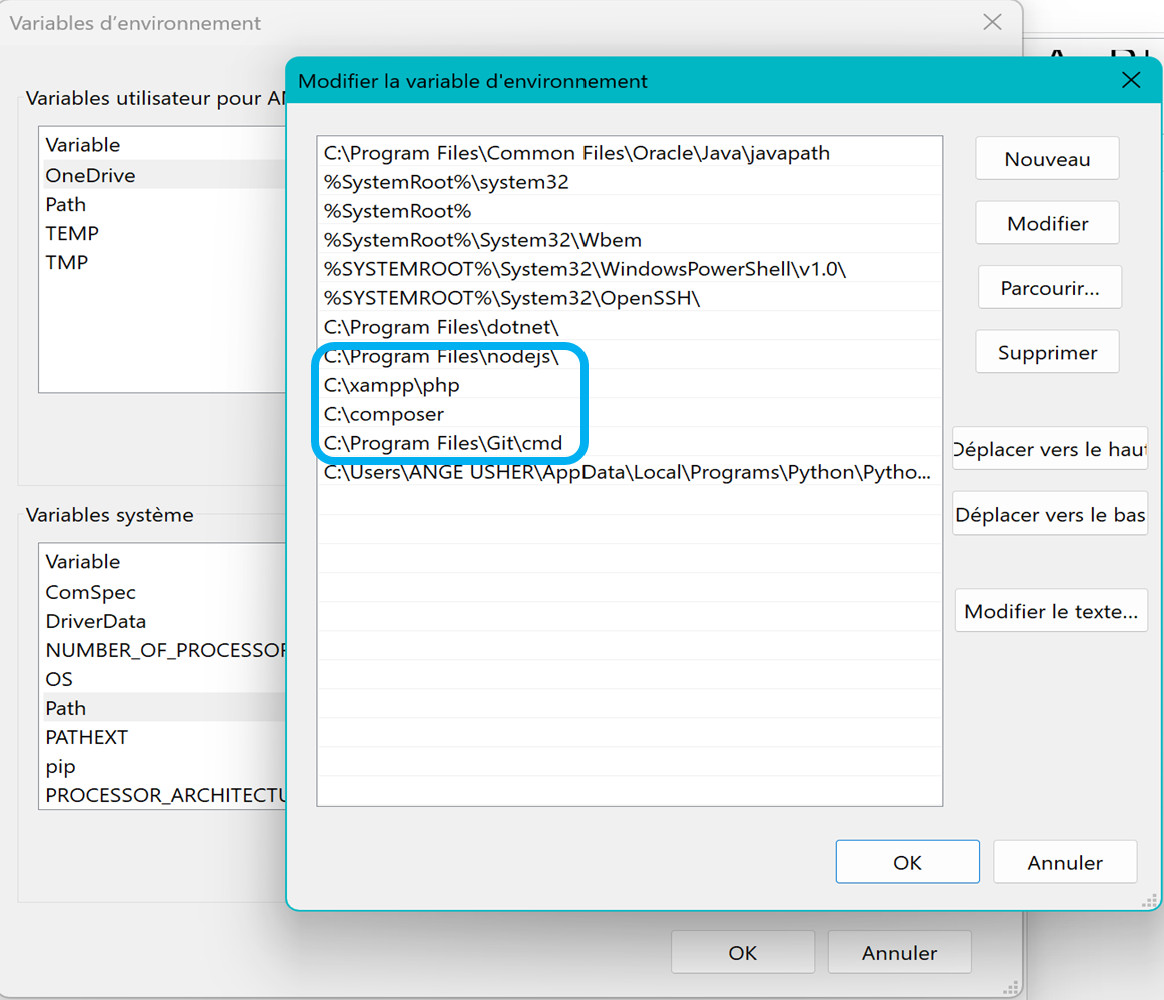
\includegraphics[width=0.58\textwidth]{./img/path.png} 
        \end{figure}

    \item \textbf{Configurer XAMPP et lancer les serveurs Apache et MySQL}
        \begin{figure}[h!] 
            \centering 
            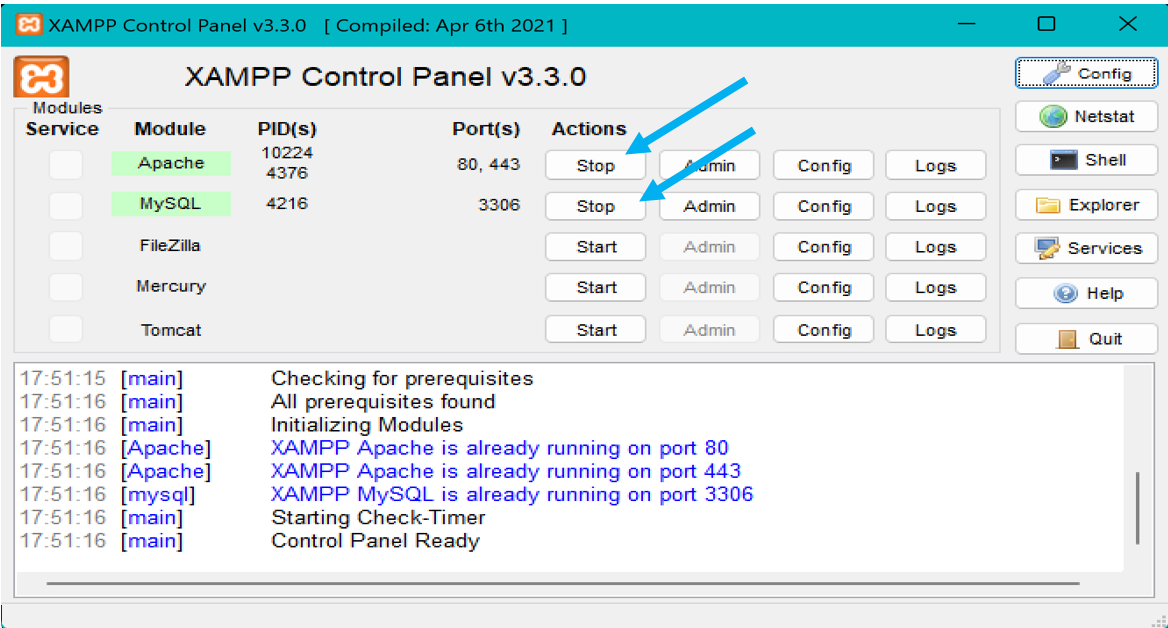
\includegraphics[width=0.7\textwidth]{./img/xampp.png} 
        \end{figure}
    \item \textbf{Créer la base de données sur MySQL}
Ouvrez PhpMyAdmin et créez-y une base de données pour l'application.
    
\rule{\linewidth}{0.2pt}
    \item \textbf{Remplacer le fichier elasticsearch.yml selon votre OS} 
Il faut procéder comme suit:
-Téléchargez Elasticsearch (depuis le site officiel) et procédez à l'extraction de l'archive dans le répertoire de votre choix (si vous ne l'aviez pas fait précédemment).

-Copiez le fichier elasticsearch.yml fourni dans le dépôt à l'emplacement de configuration d'Elasticsearch : 
        \begin{itemize}
            \item Windows :
            \begin{lstlisting}
copy config\elasticsearch\elasticsearch.yml C:\chemin\vers\elasticsearch\config\
            \end{lstlisting}
            \item Linux :
            \begin{lstlisting}
/bin/cp config/elasticsearch/elasticsearch.yml /chemin/vers/elasticsearch/config/
            \end{lstlisting}
        \end{itemize}
-Configurez le fichier elasticsearch.yml :
    \begin{lstlisting}
SCOUT_DRIVER=Matchish\ScoutElasticSearch\Engines\ElasticSearchEngine
ELASTICSEARCH_HOST=http://localhost:9200
ELASTICSEARCH_USER=elastic
ELASTICSEARCH_PASSWORD=changeme
    \end{lstlisting}
\rule{\linewidth}{0.2pt}
    \item \textbf{Lancer Elasticsearch}

Positionnez-vous sur le répertoire d'installation d'Elasticsearch et procédez au lancement.Pour ce faire, exécutez les commandes:
        \begin{lstlisting}
#  pour Windows, tapez:
cd chemin_vers_elasticsearch\bin
elasticsearch.bat
# pour Linux, tapez:
cd cd chemin_vers_elasticsearch\bin
elasticsearch
        \end{lstlisting}

Votre terminal affichera un résultat similaire à :
    \begin{figure}[h] 
        \centering 
        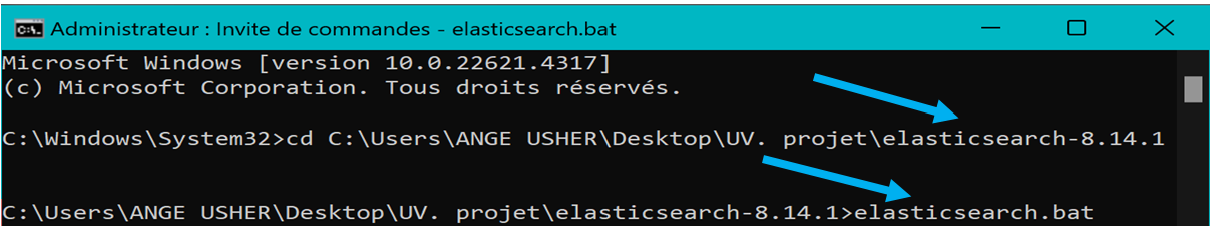
\includegraphics[width=0.8\textwidth]{./img/elastix.png} 
    \end{figure}

\rule{\linewidth}{0.2pt}
    \item \textbf{Lancer le backend Laravel}

Dans un nouveau terminal, exécutez les commandes suivantes pour vous positionner sur le répertoire du dossier backend(dossier Laravel 10 plus précisémment) et procéder au lancement:
        \begin{lstlisting}
cd chemin\vers\backend
php artisan migrate:refresh --seed
php artisan serve
        \end{lstlisting}
\rule{\linewidth}{0.2pt}
    \item \textbf{Lancer le frontend Angular}
       
Dans un nouveau terminal, exécutez les commandes suivantes pour vous positionner sur le répertoire du dossier front-end et procéder au lancement:
        \begin{lstlisting}
cd chemin\vers\frontend
ng serve
        \end{lstlisting}
L'application va commencer à builder et affichera à la fin de l'opération :
            \begin{figure}[h] 
                \centering 
                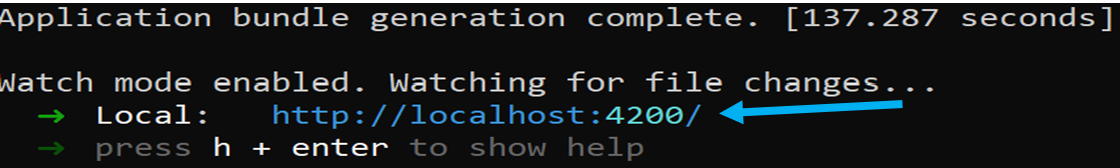
\includegraphics[width=0.8\textwidth]{./img/angular.png} 
            \end{figure}

Accéder à l'application sur :
    \begin{lstlisting}
http://localhost:4200/
    \end{lstlisting}
\end{enumerate}

\vspace{0.5cm}
\rule{\linewidth}{0.2pt}

{\fontsize{14}{16}\textbf{\textit{Problèmes courants :}}}

\begin{itemize}
    \item \textbf{Erreur de connexion à la base de données :} Vérifiez les identifiants dans `.env`.
    \item \textbf{Problème avec Elasticsearch :} Assurez-vous qu’il est bien démarré et que le numéro de port est correct.
\end{itemize}
\rule{\linewidth}{0.2pt}

\newpage
% Conclusion
{\fontsize{14}{16}\section*{Conclusion}}
\addcontentsline{toc}{section}{Conclusion}
Au vu des difficultés liées à la prise en main des applications, nous avons été appelés à mettre sur pied ce petit manuel d'assistance au déploiement de notre application. Nous y avons donc mentionné les points clés à prendre en compte pour ledit déploiement, ainsi que les difficultés que nous avons rencontrées durant cette phase. Nous espérons grandement que ce manuel vous apportera le soutient nécessaire pour y arriver sereinement. Et, dans des temps futurs, nous comptons sur l'ingéniosité des développeurs et administrateurs pour y apporter des ajustements encore plus intéressants!
\end{document}